\documentclass[12pt]{article}
\usepackage[spanish]{babel}
\usepackage{graphicx}
\usepackage{float}
\usepackage{listings}
\usepackage{xcolor}
\usepackage{tikz}

\definecolor{codegreen}{rgb}{0,0.6,0}
\definecolor{codegray}{rgb}{0.5,0.5,0.5}
\definecolor{codepurple}{rgb}{0.58,0,0.82}
\definecolor{backcolour}{rgb}{0.95,0.95,0.92}


\lstdefinestyle{mystyle}{
	backgroundcolor=\color{backcolour},   
	commentstyle=\color{codegreen},
	keywordstyle=\color{magenta},
	numberstyle=\tiny\color{codegray},
	stringstyle=\color{codepurple},
	basicstyle=\ttfamily\footnotesize,
	breakatwhitespace=false,         
	breaklines=true,                 
	captionpos=b,                    
	keepspaces=true,                 
	numbers=left,                    
	numbersep=5pt,                  
	showspaces=false,                
	showstringspaces=false,
	showtabs=false,                  
	tabsize=2
}

\lstset{style=mystyle}

\title{SISTEMAS DE CONTROL I \\ Trabajo final integrador 
	\\ Sistema de control de temperatura para un CPU}

\author{Docentes:\\ AGUERO CLAUDIO (Titular) \\ PEDRONI JUAN PABLO (Adjunto)
	\\ Alumnos: \\ Bernaus Julieta, Campos Mariano}
	
\begin{document}
	
\maketitle

\begin{abstract}
	Este proyecto tiene como objetivo diseñar e implementar un sistema de control a lazo cerrado para regular la temperatura de un CPU mediante el ajuste dinámico de la velocidad de un ventilador. El sistema busca mantener la temperatura dentro de límites seguros, optimizando el desempeño y la vida útil del CPU.
\end{abstract}\newpage

\tableofcontents \newpage

\section{Definición del problema}

	\subsection{Principio de funcionamiento del sistema}
	El sistema propuesto es un controlador a lazo cerrado para regular la temperatura de un CPU mediante el ajuste de la velocidad de un ventilador. El principio de funcionamiento se basa en la retroalimentación: se mide constantemente la temperatura del CPU, se compara con un valor deseado (setpoint), y se ajusta dinámicamente la velocidad del ventilador para mantener la temperatura en los límites establecidos.

	\subsection{Variable a controlar}
	La variable a controlar es la temperatura del CPU,($T_{CPU}$ en grados Celsius, °C). El objetivo es mantenerla dentro de un rango seguro para evitar el sobrecalentamiento, con un setpoint ajustable dependiendo de la carga del sistema.
	
	\subsection{Medición de la variable de salida}
	Si bien algunos CPU tienen incorporados sensores de temperaturas internos,para nuestro caso utilizamos un sensor de temperatura LM35.
	
	\begin{itemize}
		\item Sensor:precisión de ±0.5°C.
		\item Acondicionamiento de señal:El LM35 podría requerir un ADC si fuera necesario utiliza un microcontrolador(Se determina en las secciones posteriores).
	\end{itemize}
	
	
	
	\subsection{Ejecución de la acción de control}
	La acción de control se ejecutará mediante un ventilador de corriente continua (DC) cuyo motor será controlado con señales PWM (modulación por ancho de pulso). La señal PWM ajustará las revoluciones por minuto (RPM) del ventilador, proporcionalmente a la señal de control generada por el controlador.
	\newpage
	
	\subsection{Variables del sistema}
	\begin{table}[h!]
		\centering
		\begin{tabular}{|c|c|l|}
			\hline
			\textbf{Variable} & \textbf{Unidad} & \textbf{Descripción} \\ \hline
			$T_{CPU}$ & °C & Temperatura del CPU. \\ \hline
			$V_{Fan}$ & RPM & Velocidad del ventilador. \\ \hline
			Señal de control (u) & \% (Duty Cycle) & Señal generada por el controlador (PWM). \\ \hline
			$T_{Amb}$ & °C & Temperatura ambiente (perturbación). \\ \hline
		\end{tabular}
		\caption{Variables del sistema con sus unidades y descripciones.}
		\label{tab:variables}
	\end{table}
	
	
	\subsection{Posibles perturbaciones}
	\begin{itemize}
		\item Variaciones en la temperatura ambiente $T_{Amb}$ El sistema debe compensar los cambios en la temperatura externa.
		\item Carga del CPU: A mayor carga, se genera más calor, lo que afecta directamente la variable controlada, la $T_{CPU}$.
		\item Fluctuaciones de voltaje en el suministro eléctrico: Pueden alterar el funcionamiento del ventilador(No se tiene en cuenta para el diseño).
	\end{itemize}
	
	\subsection{No linealidades involucradas}
	El sistema de control que regula la temperatura del CPU a través del ventilador debe abordar múltiples fuentes de no linealidad:
	\begin{itemize}
		\item Ventilador: La relación entre el ciclo de trabajo PWM y la velocidad del ventilador es no lineal, especialmente a bajas RPM.
		\item Sensores de temperatura: Los sensores tienen respuestas no lineales que deben ser compensadas para obtener mediciones precisas.
		\item Transferencia de calor: El comportamiento térmico del CPU y su interacción con el sistema de enfriamiento (ventilador) es no lineal.
	\end{itemize}
	
	\subsection{Niveles de señal de entrada y salida}
	Existen dos principales señales, donde es de especial interés conocer sus rangos dinámicos, la  $T_{CPU}$ y por otro lado la señal de control $PWM$.Respecto a la primer señal tenemos que la temperatura máxima que puede alcanzar un CPU depende de varios factores, como el modelo específico del procesador, el sistema de refrigeración utilizado, y las condiciones ambientales.Se debe tener en cuenta que:
	\begin{itemize}
		\item Temperatura nominal de operación: Un CPU típico a máxima carga generalmente puede alcanzar temperaturas entre 70°C y 90°C. Este rango depende del tipo de CPU (por ejemplo, Intel o AMD), el proceso de fabricación, y las condiciones de refrigeración.
		\item Temperatura crítica o límite superior: Los fabricantes de CPUs suelen establecer una temperatura máxima segura alrededor de los 100°C a 105°C. Si el CPU alcanza estas temperaturas, el sistema activará medidas de protección, como el thermal throttling (reducción de la velocidad de reloj) o el apagado del sistema para evitar daños.
	\end{itemize}
	
	De lo mencionado anteriormente se concluye que la $T_{CPU}$ oscila entre 30°C  y 100°C, y por tanto teniendo en cuenta el datasheet del sensor LM35, el rango dinámico de la señal resulta de $300[mV]$ hasta $1[V]$ \\
	Para la segunda señal de interés tenemos la señal PWM, esta varia segun el ciclo de trabajo desde 0\% hasta el 100\%, esto se traduce en un rango dinámico de $0[V]$ (300[RPM]) hasta $5[V]$(5000[RPM]).
	 
\section{Análisis de la planta}
	 En este caso la planta es el CPU con su respectivo disipador, para obtener el modelo matemático de esta se recurre a la ley de Ohm térmica. Ademas para obtener una mejor aproximación se modela la inercia térmica de los cuerpos como una capacidad, se tiene:
	 \begin{equation}
	 	I[A]=\frac{\bigtriangleup V[V]}{R[ohm]}=Q[W]=\frac{\bigtriangleup T[Cº]}{Rth[Cº/W]}
	 \end{equation}
	 
	 \begin{equation}
	 	Cth[J/C]
	 \end{equation}
	 
	 Para la perturbación producida por la carga del CPU, esta aporta una cantidad de calor $Q[W]$ a la planta, por lo que se puede modelar con una fuente de corriente.El resultado del modelo tenemos dos flujos de calor, el entrante por la carga del CPU y el saliente debido a que $T_{CPU}<T_{CPU}$
	 
	\begin{figure}
		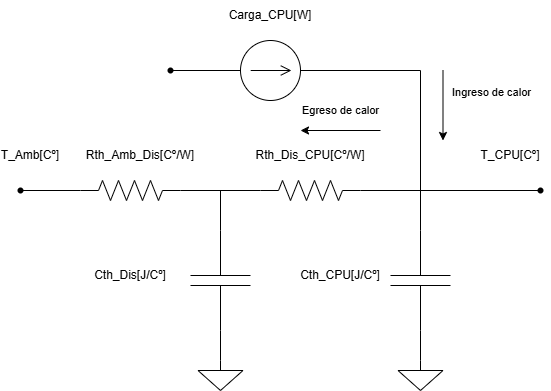
\includegraphics[width=0.9\linewidth]{Imagenes/Modelo_Planta.drawio}
		\caption[Modelo de la planta]{Modelo de la planta}
		\label{fig:modeloplanta}
	\end{figure}
	 
	 
	 
	 \subsection{Diagrama de bloques del sistema}
	 Se plantea un diagrama de bloques para modelar el sistema en su totalidad, se identifican sus partes principales(controlador, planta, sensor), las variables de entrada, salida y perturbaciones, ademas se detalla como interactúan estas entre si.
	 \begin{itemize}
	 	\item Entrada (señal de referencia):La temperatura deseada o setpoint (se puede suponer una temperatura objetivo o de referencia a mantener para el CPU, $T_{ref}$.
	 	\item Controlador: El controlador compara la temperatura medida con la temperatura de referencia y genera una señal de control en forma de PWM para el ventilador.
	 	\item Actuador: El ventilador actúa como el actuador. Recibe la señal PWM del controlador y ajusta su velocidad en función de la carga térmica del CPU.
	 	\item Perturbaciones:La temperatura ambiente y la carga del CPU son las principales perturbaciones que afectan la temperatura del CPU. Estas son fuentes de interferencia en el sistema.
	 	\item Sensor:El sensor mide la temperatura real del CPU, $T_{CPU}$ y esta señal es retroalimentada al controlador.
	 	\item Planta: El CPU es el elemento a controlar, las variables de entrada son las perturbaciones que afectan su temperatura, y la refrigeración qu aporta el ventilador, la salida es el process value $T_{CPU}$
	 \end{itemize}
	 
	\begin{figure}
		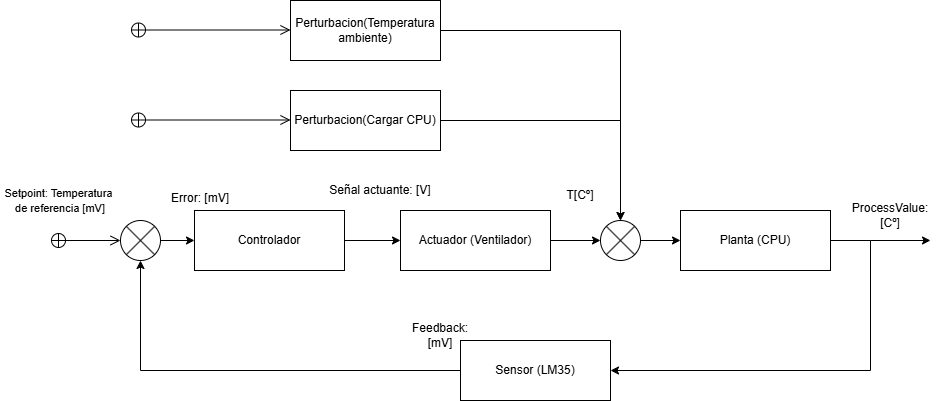
\includegraphics[width=1\linewidth]{Imagenes/diagrama_de_flujo}
		\caption[Diagrama de bloques del sistema]{Diagrama de bloques del sistema}
		\label{fig:diagramadeflujo}
	\end{figure}
	
	\subsection{Modelado matemático de los componentes}
	
		\subsubsection{Sensor de temperatura}
		En el caso de la función de transferencia del sensor de temperatura LM35,esta se puede obtener de forma teórica, ya que en el datasheet se encuentra la expresión $V_{OUT}=F(T_{Amb})$, para la aplicación típica (FIGURE 1. Basic Centigrade Temperature Sensor), la expresión resulta:
		
		\begin{equation}
			V_{OUT}[V]= 0[V]+0.01[V].T_{Amb}[°C]
		\end{equation}
		
		La función de transferencia de interés, se obtienen pasando la ecuación al dominio operacional y despejando la expresión $Voltaje/Temperatura$, esta resulta:
		
		\begin{equation}
			FdT_{Sensor}=\frac{V(s)}{T(s)}=0.01
		\end{equation}
		
		\subsubsection{Ventilador}
		Para obtener la función de transferencia del ventilador se opto por hacerlo de forma experimental, ya que la relación entrada-salida de la señal PWM y temperatura, no se encontraba disponible en ninguna bibliografía.El procedimiento es el siguiente:
		\begin{itemize}
			\item Armar el sistema de refrigeración con el ventilador y el habitáculo donde se va a encontrar el CPU.
			\item Hacer variar la señal de entrada PWM del ventilador y medir la temperatura resultante en el habitáculo.
			\item Con los datos obtenidos, mediante un script en Matlab, obtener la función de transferencia
		\end{itemize}
		
		Nota: En nuestro caso los datos son simulados con un script de python.\newpage
		
		\begin{figure}
		
			\label{fig:pwmvstemp}
			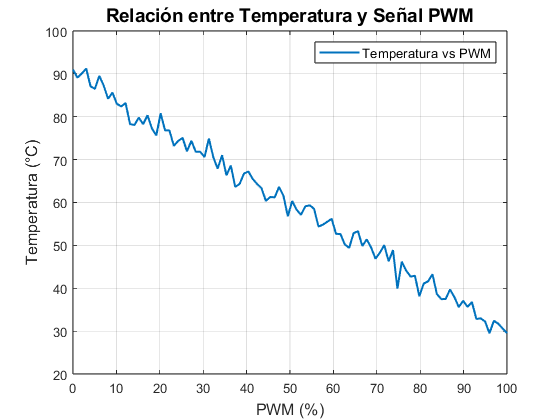
\includegraphics[width=1\linewidth]{Imagenes/pwm_vs_temp}
			\caption[Datos recopilados]{Datos recopilados}
		\end{figure}
		
		Con los datos obtenidos se realiza el siguiente análisis para obtener la función de transferencia:
		
		\begin{lstlisting}
			%Calculo de funcion de transferencias para el vantilador
			%Importamos los datos obtenidos de las mediciones
			opts = delimitedTextImportOptions("NumVariables", 2);
			opts.DataLines = [2, Inf];
			opts.Delimiter = ",";
			opts.VariableNames = ["PWM", "TemperatureC"];
			opts.VariableTypes = ["double", "double"];
			opts.ExtraColumnsRule = "ignore";
			opts.EmptyLineRule = "read";
			data = readtable("D:\GD\Sistemas de control I\Trabajo-Integrador-SCI\Datos\pwm_temperature_data.csv", opts)
			
			% Leer el archivo CSV como tabla
			data = readtable("D:\GD\Sistemas de control I\Trabajo-Integrador-SCI\Datos\pwm_temperature_data.csv",opts);
			
			% Separar las columnas en variables
			PWM = data.("PWM"); % Columna PWM
			Temperature = data.("TemperatureC"); % Columna Temperatura
			
			% Crear el grafico
			figure;
			plot(PWM, Temperature, 'LineWidth', 1.5, 'MarkerSize', 6, 'DisplayName', 'Temperatura vs PWM');
			grid on;
			xlabel('PWM (%)', 'FontSize', 12);
			ylabel('Temperatura (C)', 'FontSize', 12);
			title('Relacion entre Temperatura y Senal PWM', 'FontSize', 14);
			legend('show', 'Location', 'northeast', 'FontSize', 10);
			
			
			% Crear entrada y salida como senales en tiempo (asumiendo un muestreo uniforme)
			t = linspace(0, length(PWM)-1, length(PWM)); % Tiempo ficticio
			u = PWM; %Entrada (PWM )
			y = Temperature; % Salida (Temperatura)
			
			% Ajustar un modelo de primer o segundo orden (dominio Laplace)
			data_id = iddata(y, u, 1); % Crear datos de identificacion con un muestreo ficticio de 1s
			model = tfest(data_id, 1, 0); % Ajustar un modelo de primer orden sin ceros
			
			% Mostrar la funcion de transferencia estimada
			disp('Funcion de transferencia estimada:');
			disp(model);
			
			% Graficar comparacion entre el modelo ajustado y los datos
			figure;
			compare(data_id, model);
			title('Comparacion entre datos reales y modelo ajustado', 'FontSize', 14);
			xlabel('Tiempo (s)', 'FontSize', 12);
			ylabel('Temperatura (C)', 'FontSize', 12);
			legend('Datos reales', 'Modelo ajustado', 'Location', 'best', 'FontSize', 10);
			grid on;
		\end{lstlisting}
		
		La función de transferencia obtenida resulta:
		\begin{equation}
			FdT_{Ventilador}=\frac{-0.0038}{s+0.007}
		\end{equation}
		
	\begin{figure}[h!]
		\caption[Ajuste del modelo a partir de los datos]{}
		\label{fig:ajustemodelo}
		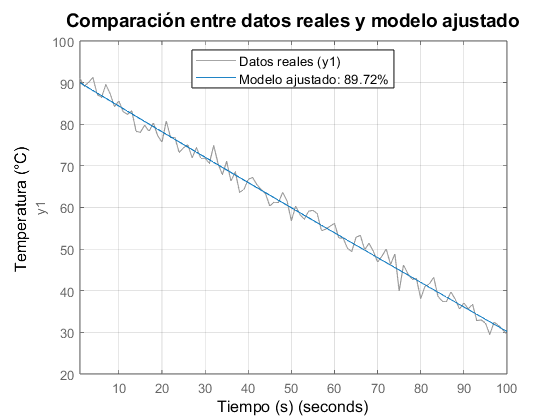
\includegraphics[width=1\linewidth]{Imagenes/ajuste_modelo}
		\caption[Ajuste del modelo a partir de los datos]{Ajuste del modelo a partir de los datos}
	\end{figure}\newpage
	
	\subsubsection{Perturbaciones}
	
		
		
	
\section{Especificaciones de diseño}

	
\section{Diseño del controlador}
\section{Simulación}
\section{Conclusiones}
\section{Bibliografía}




\end{document}
